\section{Latent Alignment Model for Lexical-Anchoring Graph-based Parsing}
\label{sec:lex-phr:graph-based}

In this section, we will introduce the two-stage framework for parsing
the DM, PSD, and AMR graphs~\S\ref{ssec:lex-phr:two-stage}. Then we
resolve the alignment problem with a latent alignment model~\S\ref{ssec:lex-phr:latent-alignment}


According to the linguistic analysis on anchoring, we have shown that
DM, PSD and AMR belong to the lexical-anchoring, which indicates that
their nodes in the output graph are explicitly or implicitly anchored
to the lexical units of the corresponding input sentence.  Before
showing the unified design of independent factorization, let us
introduce the fundamental concepts and notations.

We refer to words in a sentence as
$x=(x_{0};x_{1};...x_{i};...;x_{n})$, where $n$ is the sentence
length.  For all the graph-based representations in our
lexical-anchoring category, we decompose the whole graph into nodes
and edges. We denotes the labelled nodes~(concepts) as
$C = \{c_{i}\mid i \in [0,m]\}$, where $m$ is the number of concepts.
While the labelled edges~(relations) between the $m$ concepts are
denoted as $R = \{r_{ij}\mid i \in [0, m], j \in [0, m]\}$.  $r_{ij}$ means
the directional relation from the node $i$ to the node $j$.  We use
$r_{ij}=\Phi$ to indicate no edge from the node $i$ to the node $j$.

In this part, based on the above notations, we introduce how to do
independent factorization on lexical-anchoring by addressing the three
main chellenges in \textbf{Output
  Decomposition}~(\S\ref{sssec:lex-phr:lex-output-decomposition}),
\textbf{Input Decomposition and Alignments
  Discovery}~(\S\ref{sssec:lex-phr:lex-input-decomposition}), and
\textbf{Factor Modelling}~(Two-stage
Parsing~\S\ref{ssec:lex-phr:two-stage} and Latent Alignment
Model~\S\ref{ssec:lex-phr:latent-alignment})

\subsection{Independent Factorization on Lexical Anchoring}
\label{ssec:lex-phr:lex-factorization-analysis}
In the following, we focus on the first two main challenges in
independent factorization: \textbf{output decomposition} and
\textbf{input decomposition} on lexical-anchoring representations. We leave the
\textbf{factor modelling} into the next part.  We take a more
complicated AMR graph in~\autoref{fig:bg:amr} as an example, for the
sentence, \kw{Pierre Vinken, 61 years old, will join the board as a
  nonexecutive director Nov.29.} We introduce the details of
independent factorization for AMR and other lexical-anchoring
representations.

%\begin{figure}[t]
%\centering
%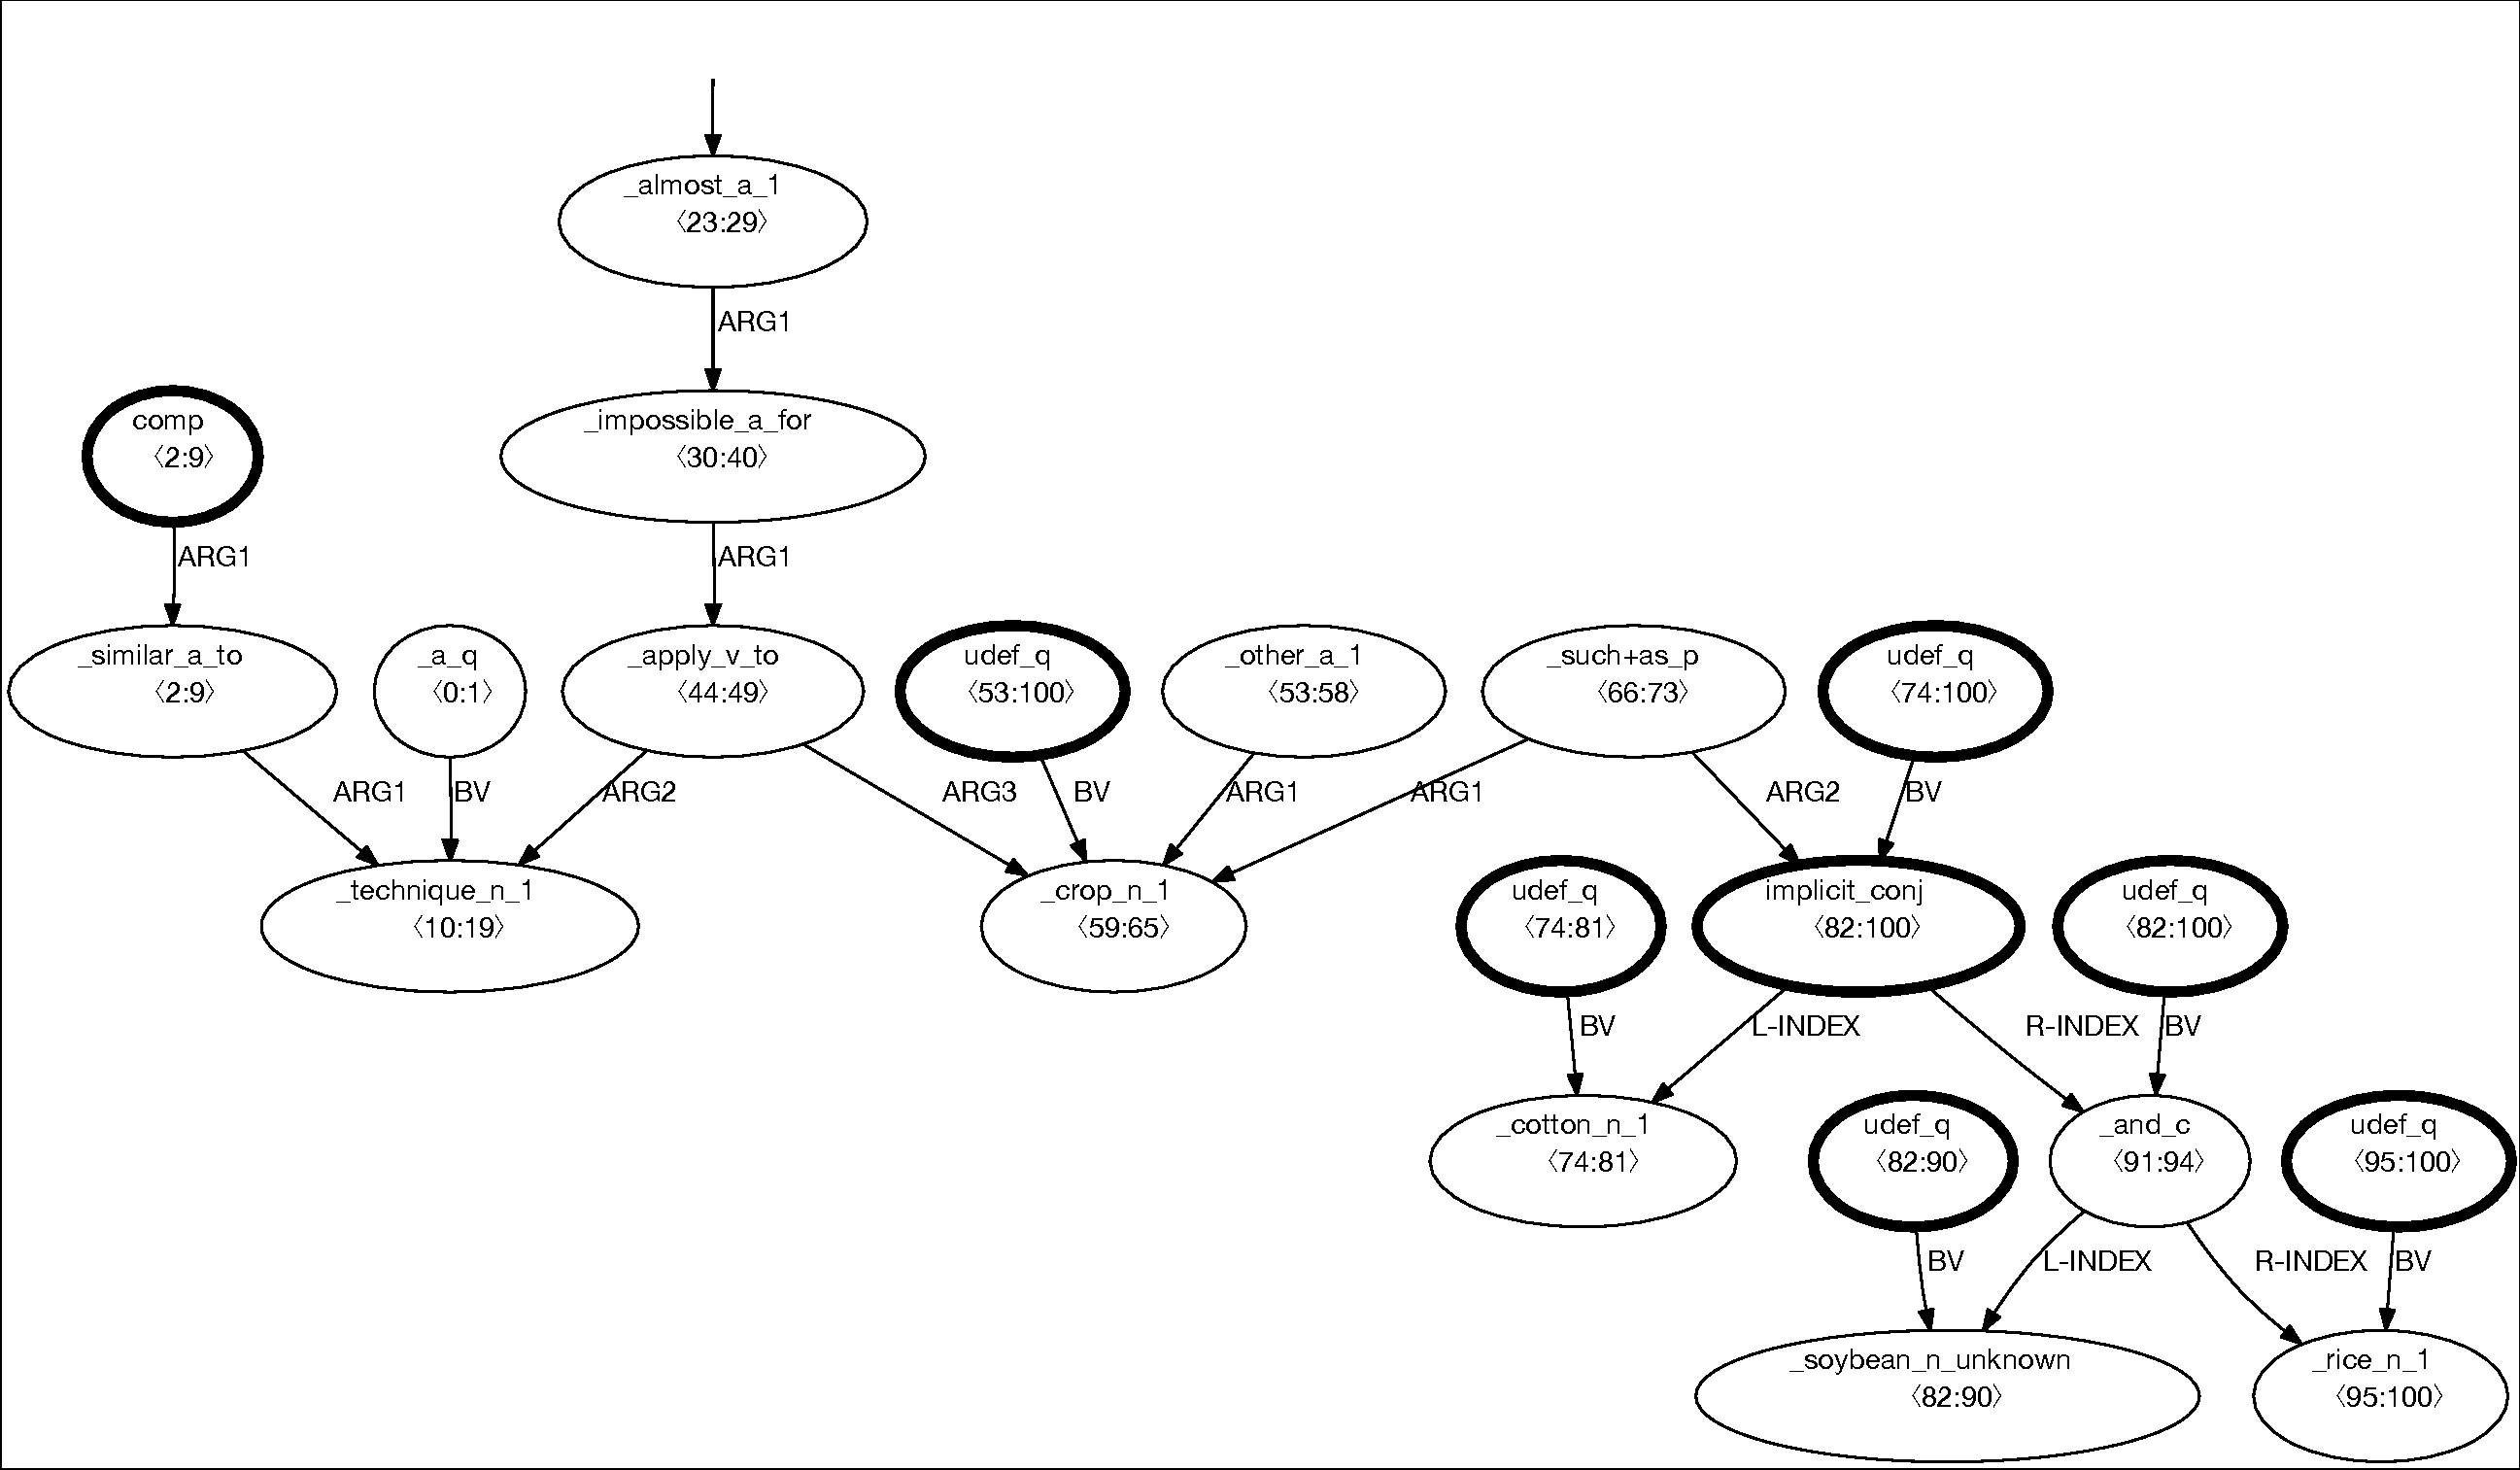
\includegraphics[width=.96\textwidth,trim=.1cm .1cm .05cm .05cm, clip]{eds-white.pdf}
%\caption{\label{fig:phrasal-anchoring}Phrasal-anchoring in
%  EDS[wsj\#0209013], for the sentence \texttt{\char`\"A similar
%    technique is almost impossible to apply to other crops, such as
%    cotton, soybeans and rice.\char`\"}. Bold nodes are similar to the
%  non-terminal nodes in UCCA, which are anchored multiple tokens, thus
%  overlapping with the anchors of other nodes.}
%\end{figure}

\subsubsection{Output Decomposition}
\label{sssec:lex-phr:lex-output-decomposition}
For the lexical-anchoring graph-based representations~(DM, PSD, AMR),
the target graph can be decomposed into independent nodes or
subgraphs. For DM and PSD, each node in the target graph is strictly
aligned to the corresponding token. Hence, we simply decompose the DM
and PSD graph by nodes. However, when we introduce the necessary of
structural inductive biases for independent
factorization~(\autoref{sssec:intro:structural-biases}), the AMR
parsing running examples shows that we need to handle those special
entities in AMR graph.  From the training data alone, we cannot easily
tell how to segment the AMR graphs. However, according to the
annotation guideline of AMR and previous work on subgraph
templating~\cite{Werling:2015up} or abstract concept
label~\cite{Wang:2017vt}, the main intuition of grouping is to ensure
that concepts are rarely lexically triggered (\eg, \tquoted{person}
and \dquoted{have-org-role-91} in~\autoref{fig:bg:amr} get grouped
together with lexically triggered nodes~(\eg, \tquoted{Pierre
  Vinken} and \dquoted{director}). Finally, we adopt the templates
proposed by~\citet{lyu2018amr} including: \textbf{thing}~(\eg,
\tquoted{(opine-01 :ARG-01 thing)} for \tquoted{opinion}),
\textbf{person}~(\eg, \tquoted{(play-01 :ARG1 person)} for
\tquoted{player}), \textbf{more}, \textbf{most}~(\eg,
\tquoted{(have-degree-91 :ARG2 good-02) :ARG3 more)} for
\tquoted{better}), \textbf{date-entity}~(\eg,~\tquoted{(date-entity
  :month 2)} for \tquoted{February}), and all the \textbf{special quantity
entities}, \textbf{xx-quantity}~(\eg, \tquoted{(monetary-quantity
  :quant 20 :unit dollar)} for \tquoted{\$20}).~\footnote{Please refer
  to the paper of~\citet{lyu2018amr} for more details about the
  recategorization.} AMR output decomposition will be the rectangled segments shown in
\autoref{fig:lex-phr:amr-decomposition}.
\begin{figure}[!tbp]
  \begin{center}
  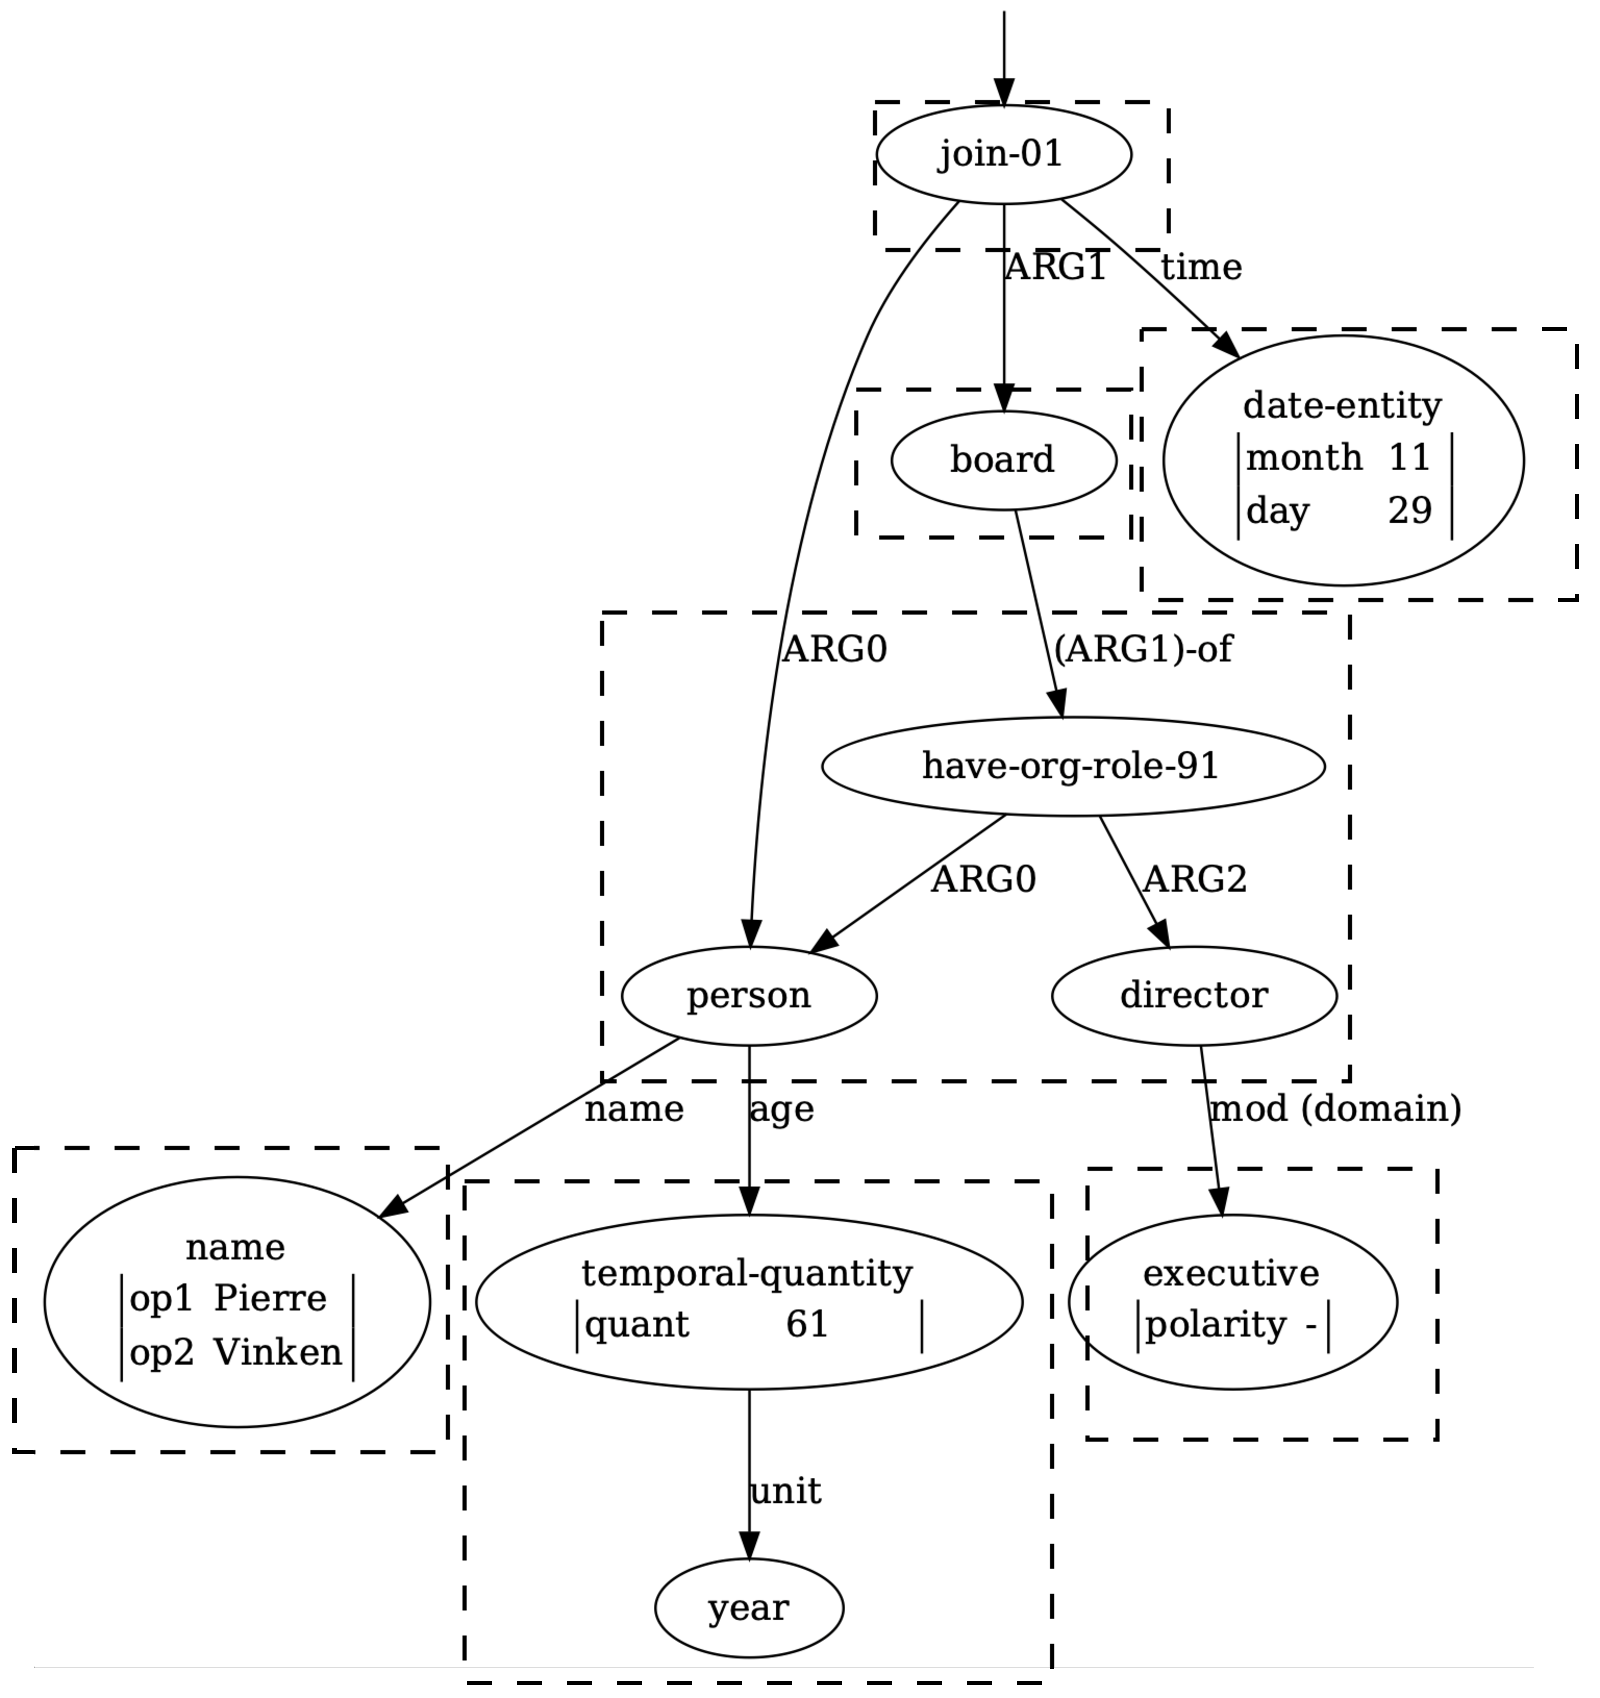
\includegraphics[width=0.90\textwidth]{pierre-decomposition.pdf}
  \end{center}
  \caption{\label{fig:lex-phr:amr-decomposition} AMR output
    decomposition for the sentence \#20001001.}
\end{figure}

\subsubsection{Input Decomposition and Alignments Discovery}
\label{sssec:lex-phr:lex-input-decomposition}

According to the bilexical dependency structures of DM and PSD, and
implicit lexical token anchoring on AMR, the nodes or categorized graph
fragments in DM, PSD, and AMR are anchored to surface lexical units in
an explicit or implicit way. Especially, those lexical units do not
overlap with each other, and most of them are just single-tokens,
multiple word expression, or named entities. In other words, when
parsing a sentence into DM, PSD, AMR graphs, and tokens in the original
sentence can be merged by looking up a lexicon dict when preprocessing
and then may be considered as a single token for aligning or parsing.

The more difficult challenge exists in how to align the decomposed
input with the decomposed output. According to the previous anchoring
analysis, the training data of DM and PSD naturally contains the
anchoring information, while the AMR training data doesn't offer the
alignments. Hence, for AMR, we need to an extra model to resolve the
alignments discovery problem. According to the AMR annotation
guideline, a strong inductive bias about the alignment is that
\emph{each token or expressive is not overlapping and is
  exclusively aligned to the output decompositions.} We will
introduce the details of the latent alignment model in
\autoref{ssec:lex-phr:latent-alignment}.

%%% Local Variables:
%%% mode: latex
%%% TeX-master: "../../dissertation-main.ltx"
%%% End:


\subsection{Two-stage Graph-Based Parsing}
\label{ssec:lex-phr:two-stage}

Before formulating the graph-based model into a probabilistic model as
Equation \ref{eq:graph_prob}, we denote some notations: $C$, $R$ are
sets of concepts (nodes) and relations (edges) in the graph, and $w$
is a sequence of tokens.  $a \in {\mathbb{Z}}^m$ as the alignment
matrix, each $a_{i}$ is the index of aligned token where $i$th node
aligned to. When modeling the negative log likelihood loss~(NLL), with
independence assumption between each node and edge, we decompose it
into node- and edge-identification pipelines.

\begin{equation}
  \label{eq:graph_prob}
\begin{aligned} \smaller[2]
 & NLL(P(C,R \mid w)) \\
 & = - \log(P(C,R \mid w)) \\
 & = - \log(\sum_{a}{P(a) P(C,R \mid w,a)}) \\
 & = - \log\left(\sum_{a}P(a) P(R\mid w,a,C) P(C \mid w, a)\right) \\
 & = - \log\left(\sum_{a}P(a) \prod_{i}^{m} P(c_{i} \mid h_{a_{i}}) \right. \\
 & \qquad \left.\cdot \prod_{i,j=1}^{m}P(r_{ij} \mid h_{a_{i}}, c_{i}, h_{a_{j}}, c_{j})\right)
\end{aligned}
\end{equation}

In DM, PSD, and AMR, every token will only be aligned once.  Hence, we
train a joint model to maximize the above probability for both node
identification
$P(c_{i} \mid h_{a_{i}})$~\S\ref{sssec:lex-phr:node-ident} and edge
identification
$P(r_{ij} \mid h_{{a_{i}}, c_{i},h_{a_{j}},
  c_{j}})$~\S\ref{sssec:lex-phr:edge-ident}. The alignment
information is mainly used for training. We need to marginalize out
the discrete alignment variable $a$ to jointly learning the parameters
in node identification and relation identification networks. We will
introduce the latent alignment model
in~\autoref{ssec:lex-phr:latent-alignment}. \autoref{fig:graph-based-inference}
summerize the unifed two-stage graph based parsing framework. In the
following subsections, we will explain the framework in more details.

\begin{figure}[h] \centering
  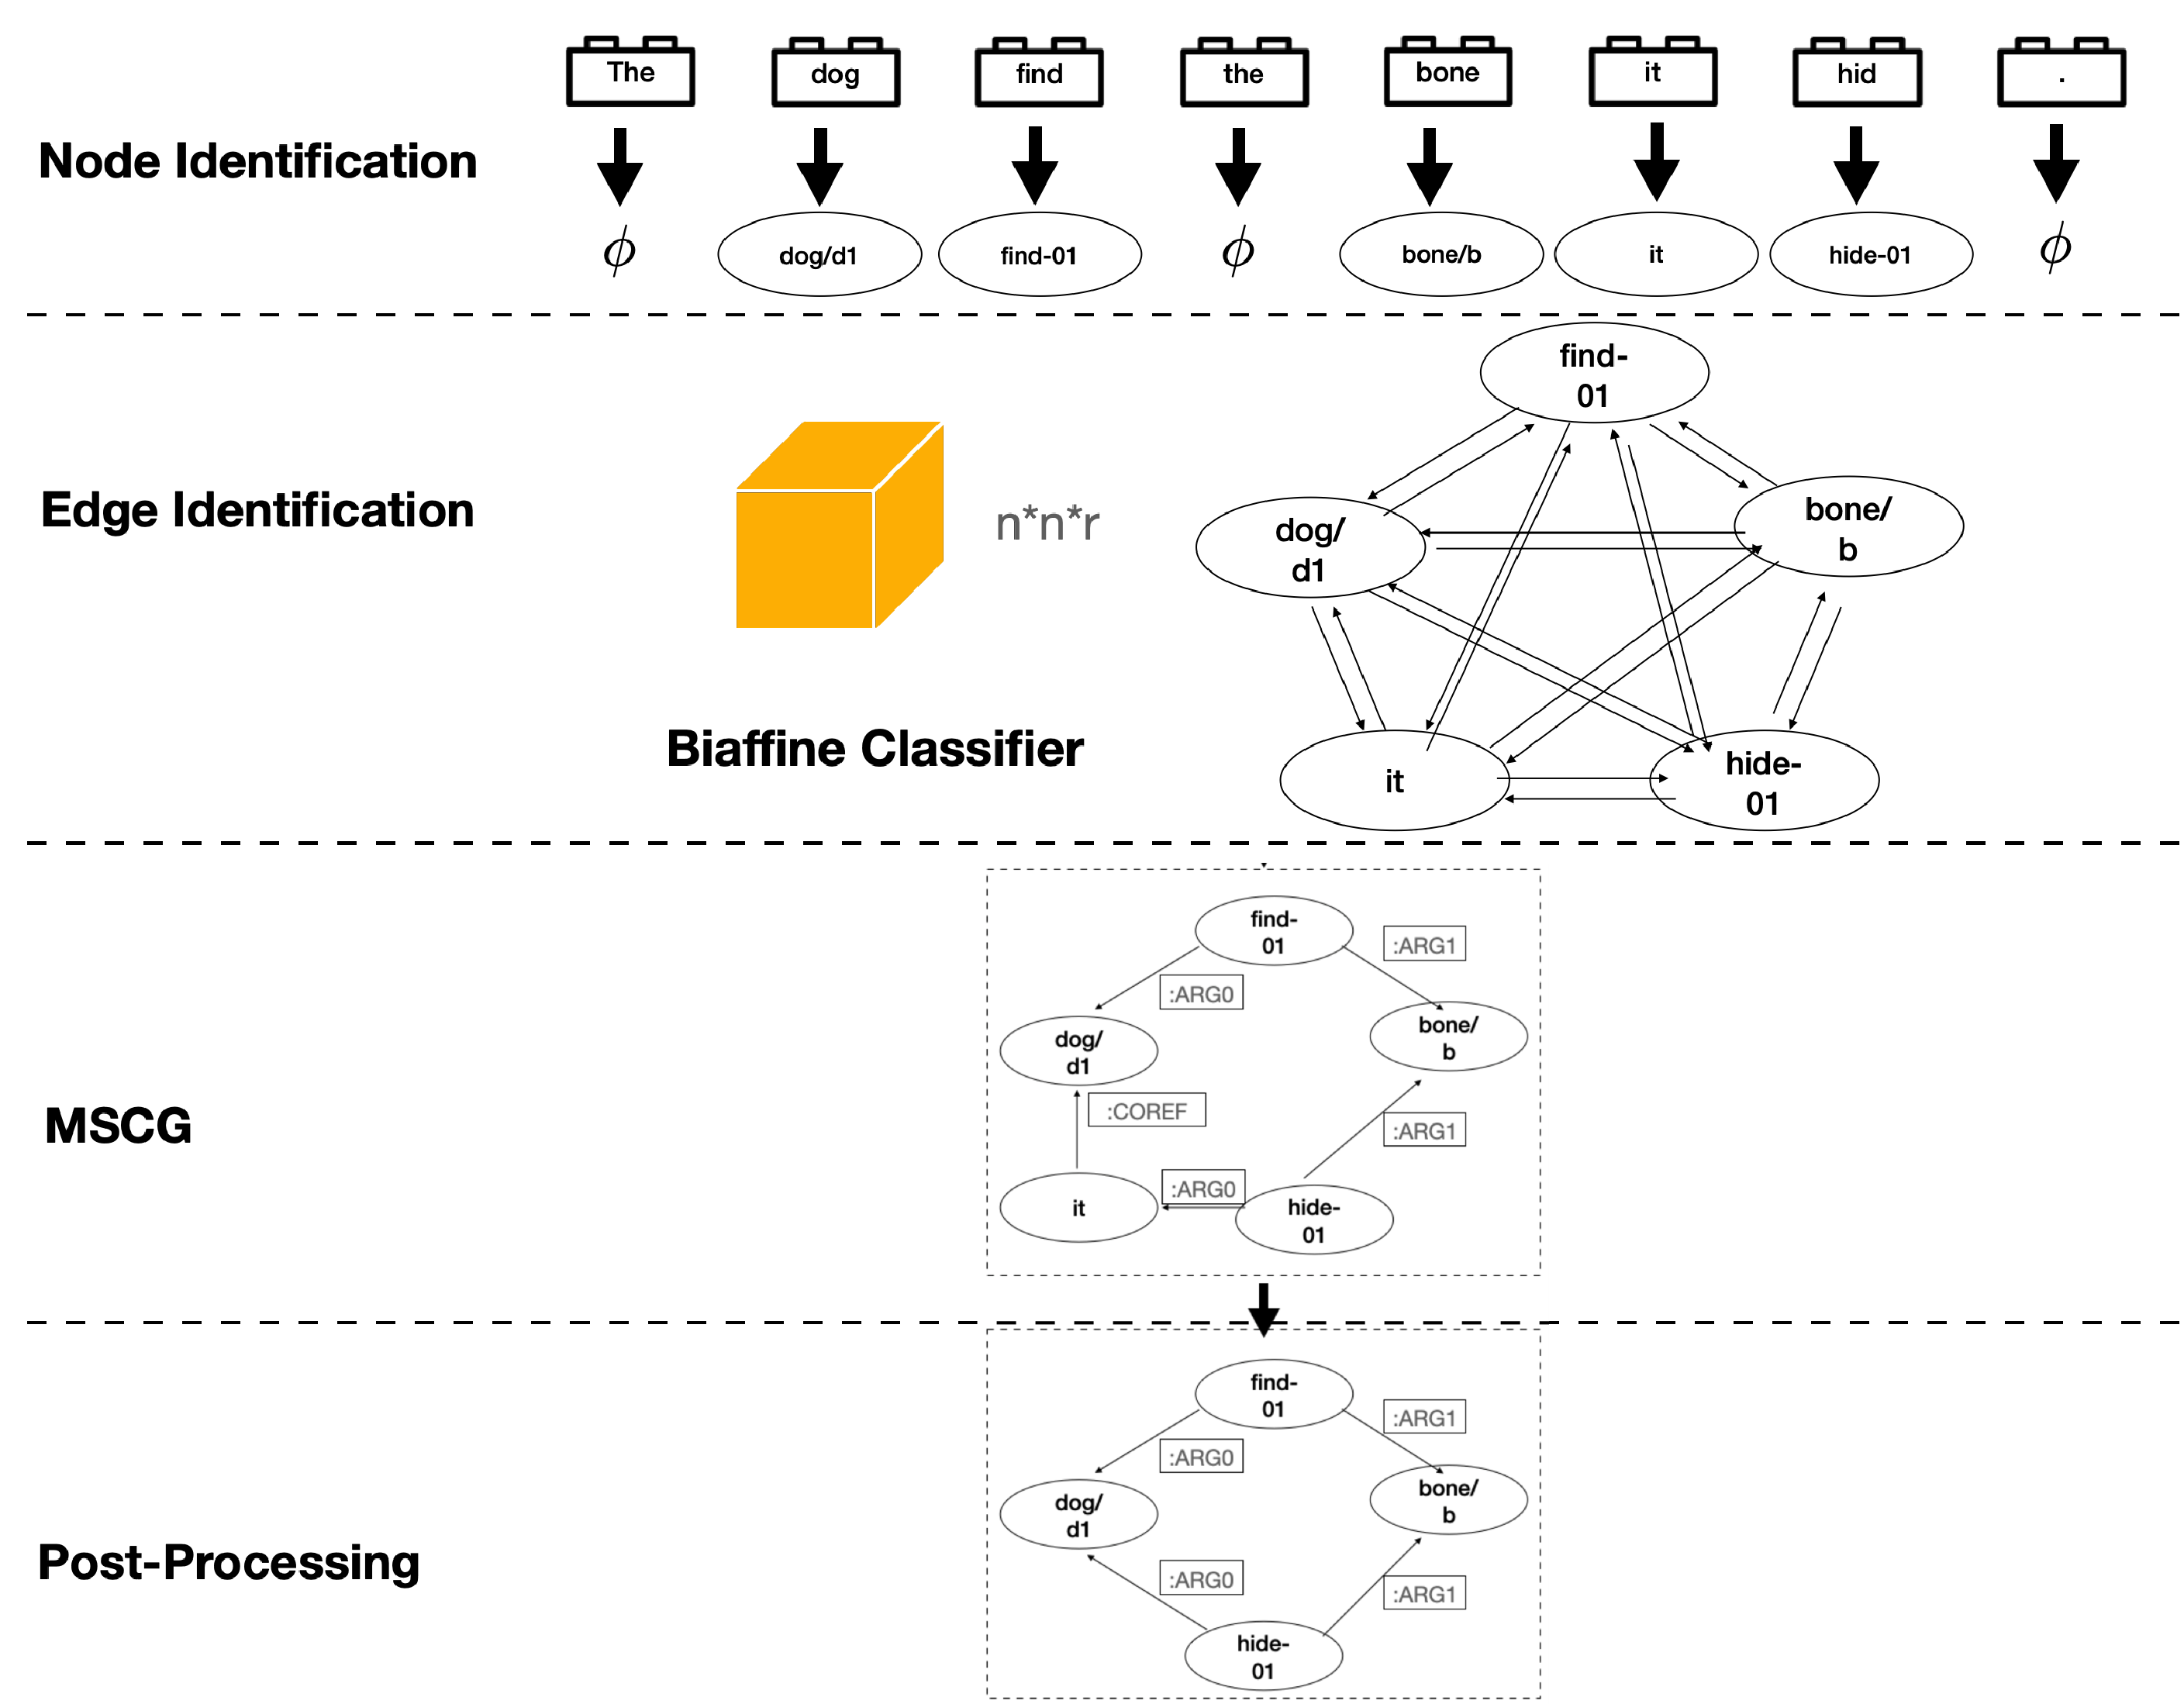
\includegraphics[width=1.00\textwidth]{graph-overview3.pdf}
  \caption{\label{fig:graph-based-inference} Two-stage graph-based
    parsing for the running exmaple [wsj\#0209013]}
\end{figure}

\subsubsection{Node Identification}
\label{sssec:lex-phr:node-ident}
Node Identification predicts a concept $c$ given a word. A
concept can be either {\it NULL} (when there is no semantic node
anchoring to that word, e.g., the word is dropped), or a node label
(e.g., lemma, sense, POS, name value in AMR, frame value in PSD), or
other node properties. One challenge in node identification is the
data sparsity issue. Many of the labels are from open sets derived
from the input token, e.g., its lemma.  Moreover, some labels are
constrained by a deterministic label set given the word. Hence, we
designed a copy mechanism~\citep{luong2014addressing} in our neural
network architecture to decide whether to copying deterministic label
given a word or estimate a classification probability from a fixed
label set.


\subsubsection{Edge Identification}
\label{sssec:lex-phr:edge-ident}

By assuming the independence of each edge, we model the edges
probabilites independently.  Given two nodes and their underlying
tokens, we predict the edge label as the semantic relation between the
two concepts with a bi-affine classifier~\cite{dozat2016deep}.

\subsubsection{Inference}
\label{sssec:lex-phr:inference}
In our two-stage graph-based parsing, after nodes are identified, edge
identification only output a probility distribution over all the
relations between identified nodes. However, we need to an inference
algorithm to search for the \kw{maximum spanning connected graph} from all
the relations. We use~\citet[MSCG,][]{Flanigan:2014vc} to greedily
select the most valuable edges from the identified nodes and their
relations connecting them. As shown in Figure
\ref{fig:graph-based-inference}, an input sentence goes through
preprocessing, node identification, edge identification, root
identification, and MCSG to generate a final connected graph as
structured output.

\subsection{Latent Alignment Model}
\label{ssec:lex-phr:latent-alignment}

As the two-stage probablistic model shown
in~\autoref{eq:graph_prob_brief}, we need to marginalize all the
alignment information $a$ to learn the above two-stage nerual networks
for node and edge identification. We do the following computing for
explicit and implicit alignments respectively.

\Paragraph{Explicit Alignments} For DM, PSD, with explicit alignments
$a*$, we can simply use $P(a^{*}) = 1.0$ and other alignments
$P(a | a \neq a^{*}) = 0.0 $. In this case, with known alignment
information, we don't need to worry the marginalization problem.

\Paragraph{Implicit Alignments} However, For AMR, without gold
alignments, one requires to compute all the valid alignments and then
condition the node- and edge-identification methods on the alignments.
However, it is computationally intractable to enumerate all
combinatoral values for the discrete alignment variable. Hence, we
estimate the latent alignments via variational inferece, which has
been initialially used in \citet{lyu2018amr}. In the following
section, we firstly introduce the details of latent alignment model
via continuous relaxiation~\S\ref{sssec:lex-phr:alignment-relax} and
then we descibe the details of variational
inference~\S\ref{sssec:lex-phr:gumble-sinkhorn}, and we propose a
error fix for computing KL-divergence with implicit Gumbel-Sinkhorn
distribution.

\begin{equation}
  \label{eq:graph_prob_brief}
\begin{aligned} \smaller[2]
 & NLL(P(C,R \mid w)) \\
 & = - \log\left(\sum_{a}P(a) \prod_{i}^{m} P(c_{i} \mid h_{a_{i}}) \right. \\
 & \qquad \left.\cdot \prod_{i,j=1}^{m}P(r_{ij} \mid h_{a_{i}}, c_{i}, h_{a_{j}}, c_{j})\right)
\end{aligned}
\end{equation}

\subsubsection{Continuous Relaxation for Discrete Alignments}
\label{sssec:lex-phr:alignment-relax}

\begin{equation}
 \label{eq:elbo}
\begin{aligned} \smaller[2]
  & \log(P(C,R \mid w)) \geq \\
  & E_{Q}[\log(P_{\theta}(c\mid w,a) P_{\Phi}(R\mid w,a,c))] \\
  & - \kld{Q_{\Psi}(a\mid c, R,w)}{P(a)}
\end{aligned}
\end{equation}

\subsubsection{VAE, Perturb-and-Map, Gumble Sinkhorn}
\label{sssec:lex-phr:gumble-sinkhorn}
\begin{itemize}
\item Applying variational inference to reduce it into
  Evidence Lower Bound~\cite[ELBO,][]{kingma2013auto}
\item The denominator $Z_{\Psi}$ in Q can be estimated by Perturb-and-Max(MAP)~\cite{papandreouperturb}
\begin{equation}
  \label{eq:posterior_prob}
\begin{aligned} \smaller[2]
Q_{\Psi}(a\mid c, R,w)= \frac{\exp(\sum_{i=1}^{n} \phi(g_{i}, h_{a_{i}}))} {Z_{\Psi}(c,w)}
\end{aligned}
\end{equation}
Where $\phi(g_{i}, h_{a_{i}})$ score each alignment link between node i and the corresponding words,
$g_{i}$ is node encoding, and $h_{a_{i}}$ is encoding for the aligned token.

\item Discrete \texttt{argmax} of a permutation can be estimated by
  Gumbel-Softmax Sinkhorn Networks \cite{mena2018learning, lyu2018amr}
\end{itemize}

%%% Local Variables:
%%% mode: latex
%%% TeX-master: "../../thesis-main.ltx"
%%% End:
